\chapter{Byers, first module}





\begin{figure}[h!]
    \centering
    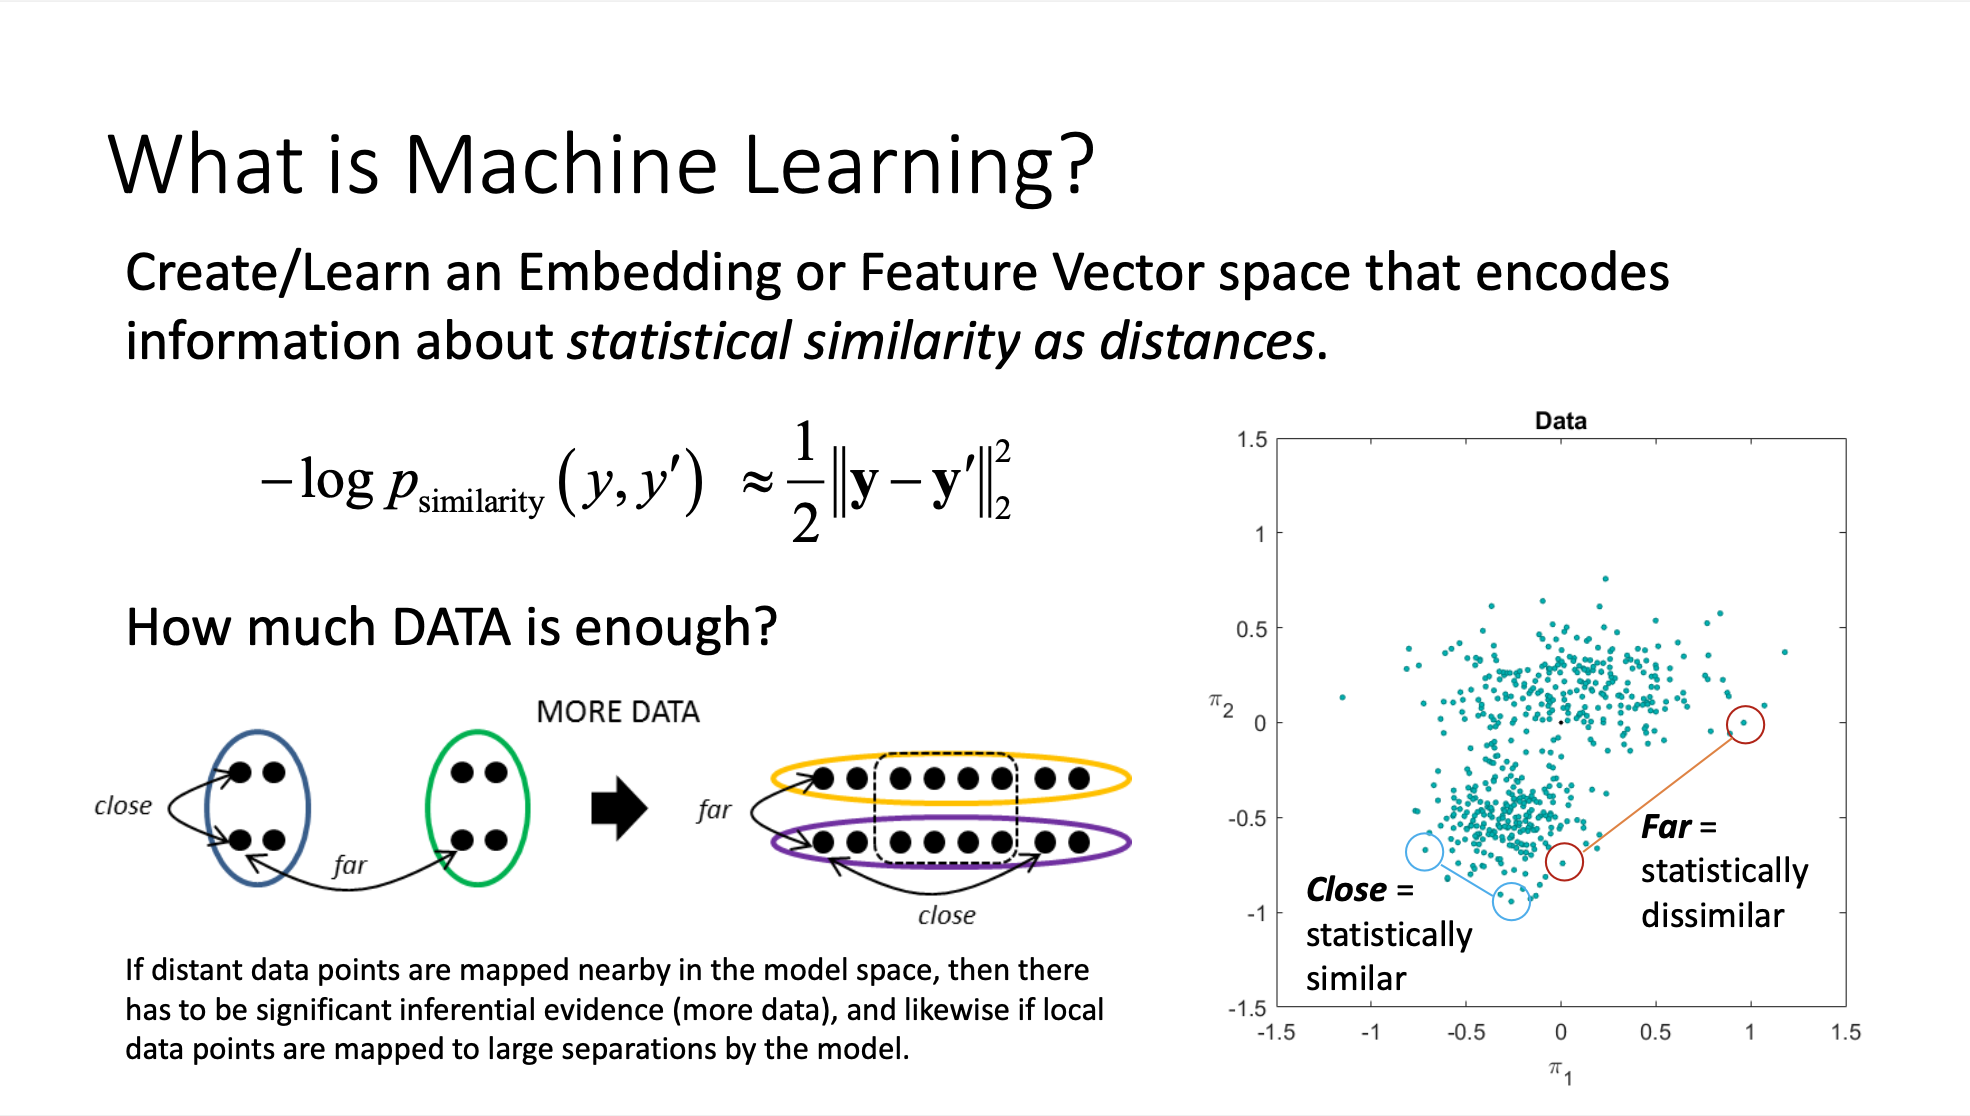
\includegraphics[width=\textwidth]{figures/B1_self_information_potential.png}
    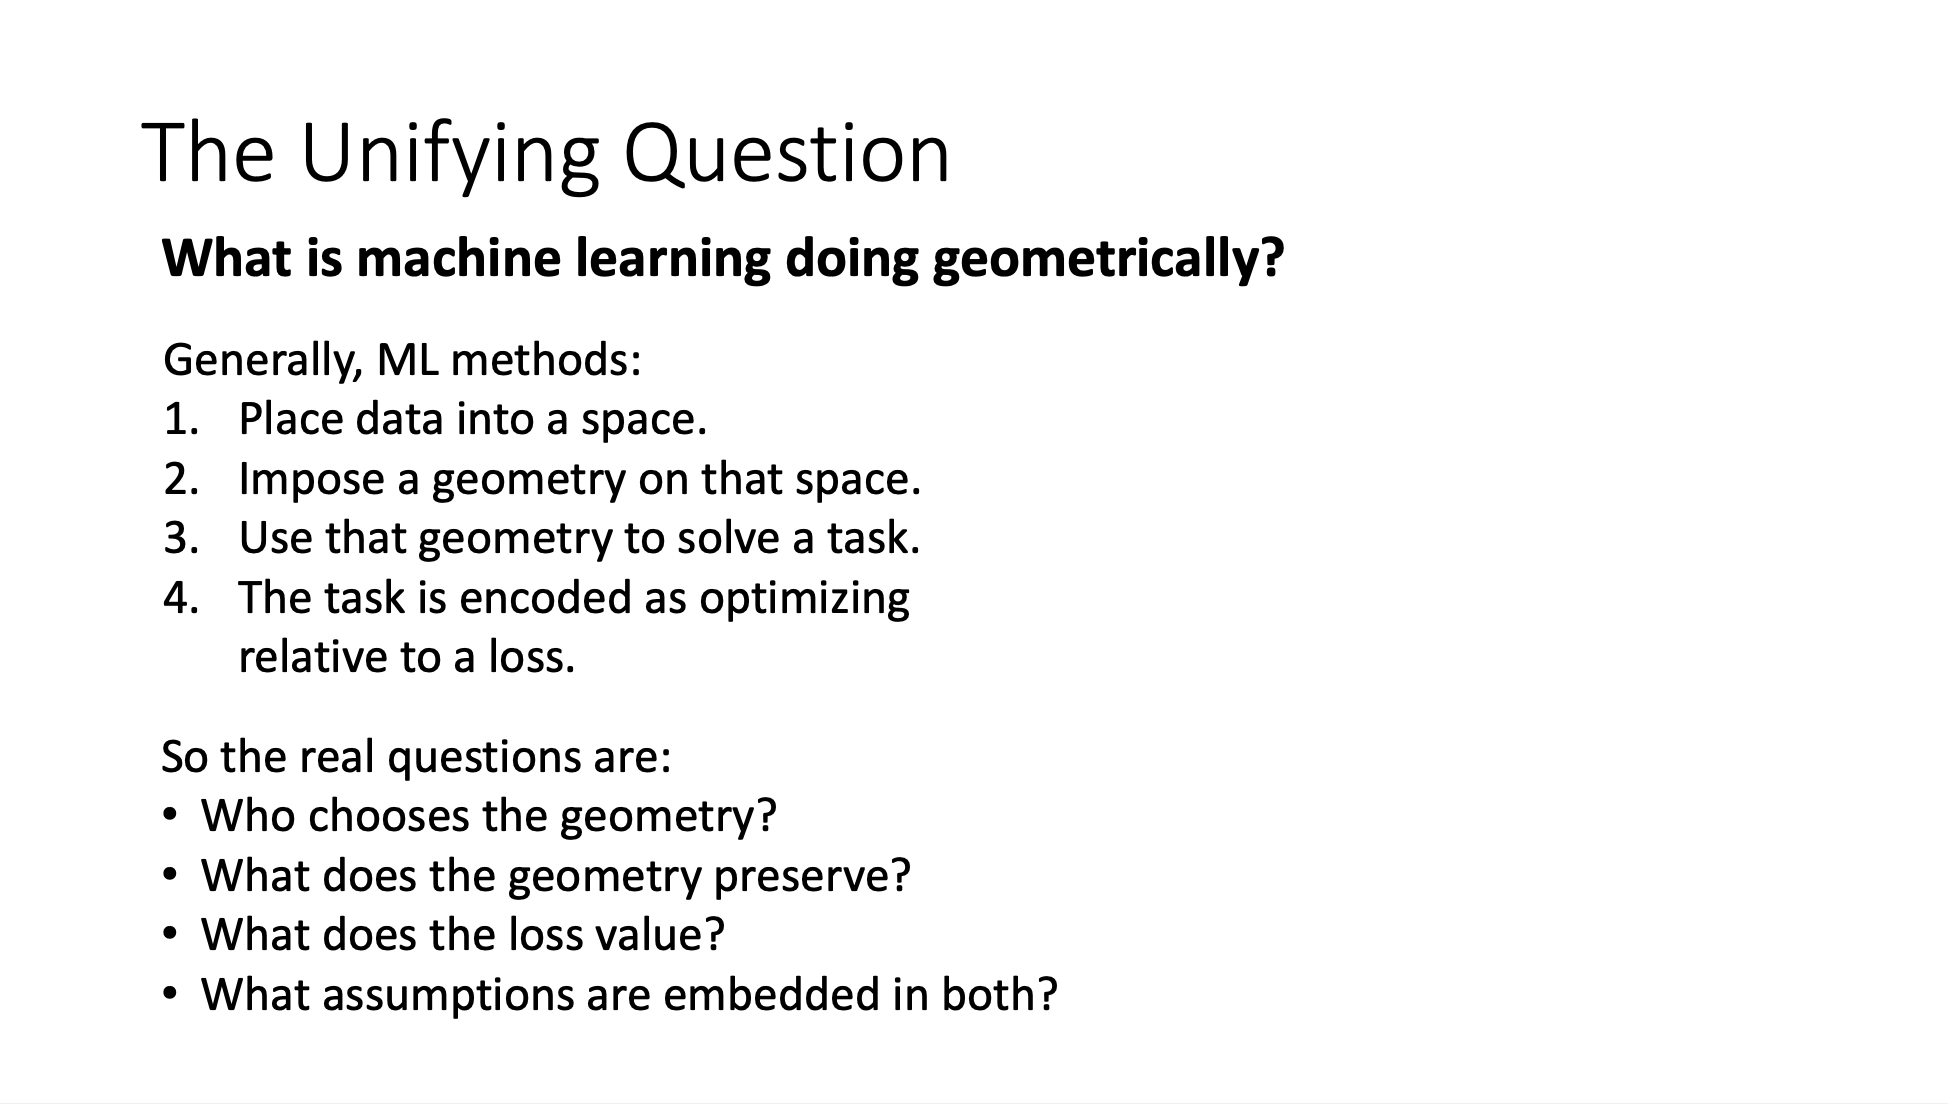
\includegraphics[width=\textwidth]{figures/B1_the_unifying_question.png}
    \caption{Self-information potential}
    \label{fig:self_information_potential}
\end{figure}


\begin{figure}[h!]
    \centering
    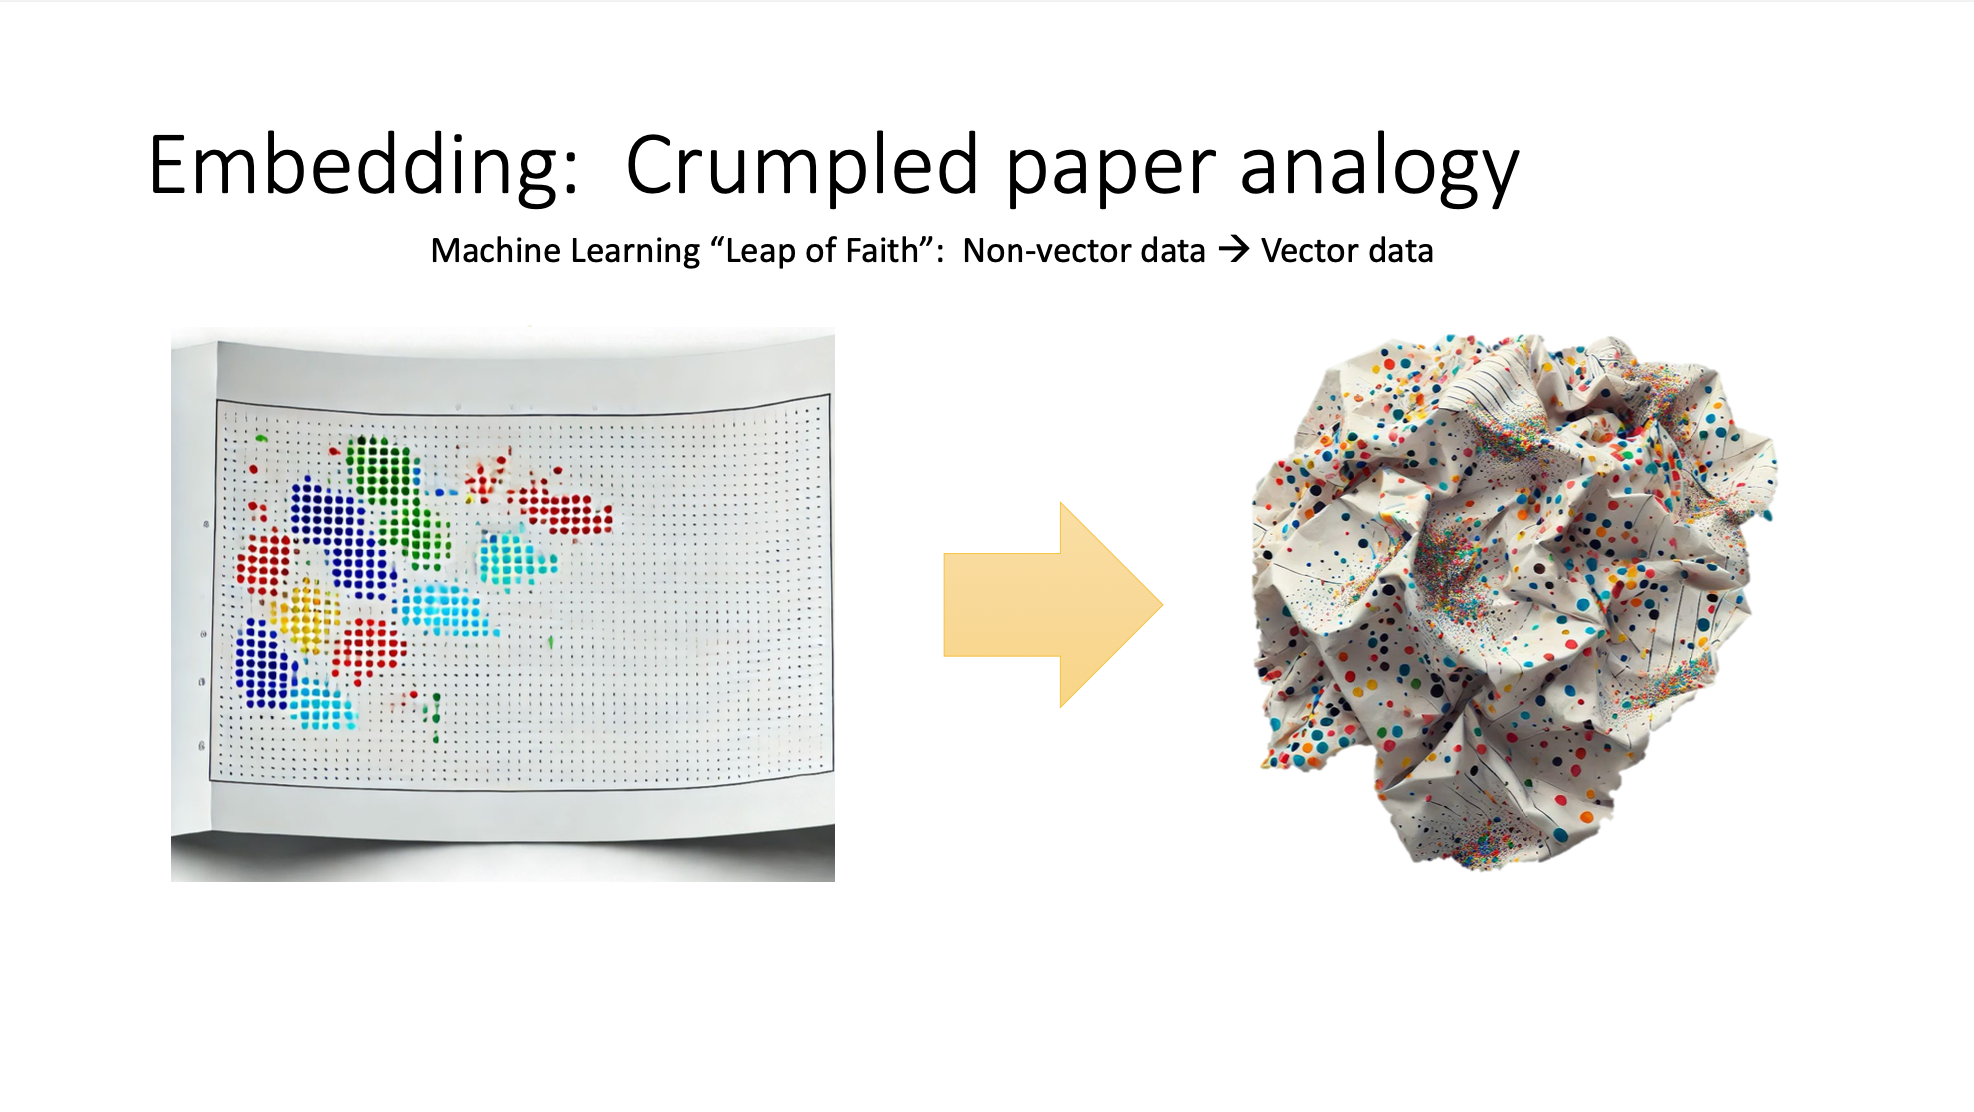
\includegraphics[width=0.8\textwidth]{figures/B1_crumbled_paper.png}
    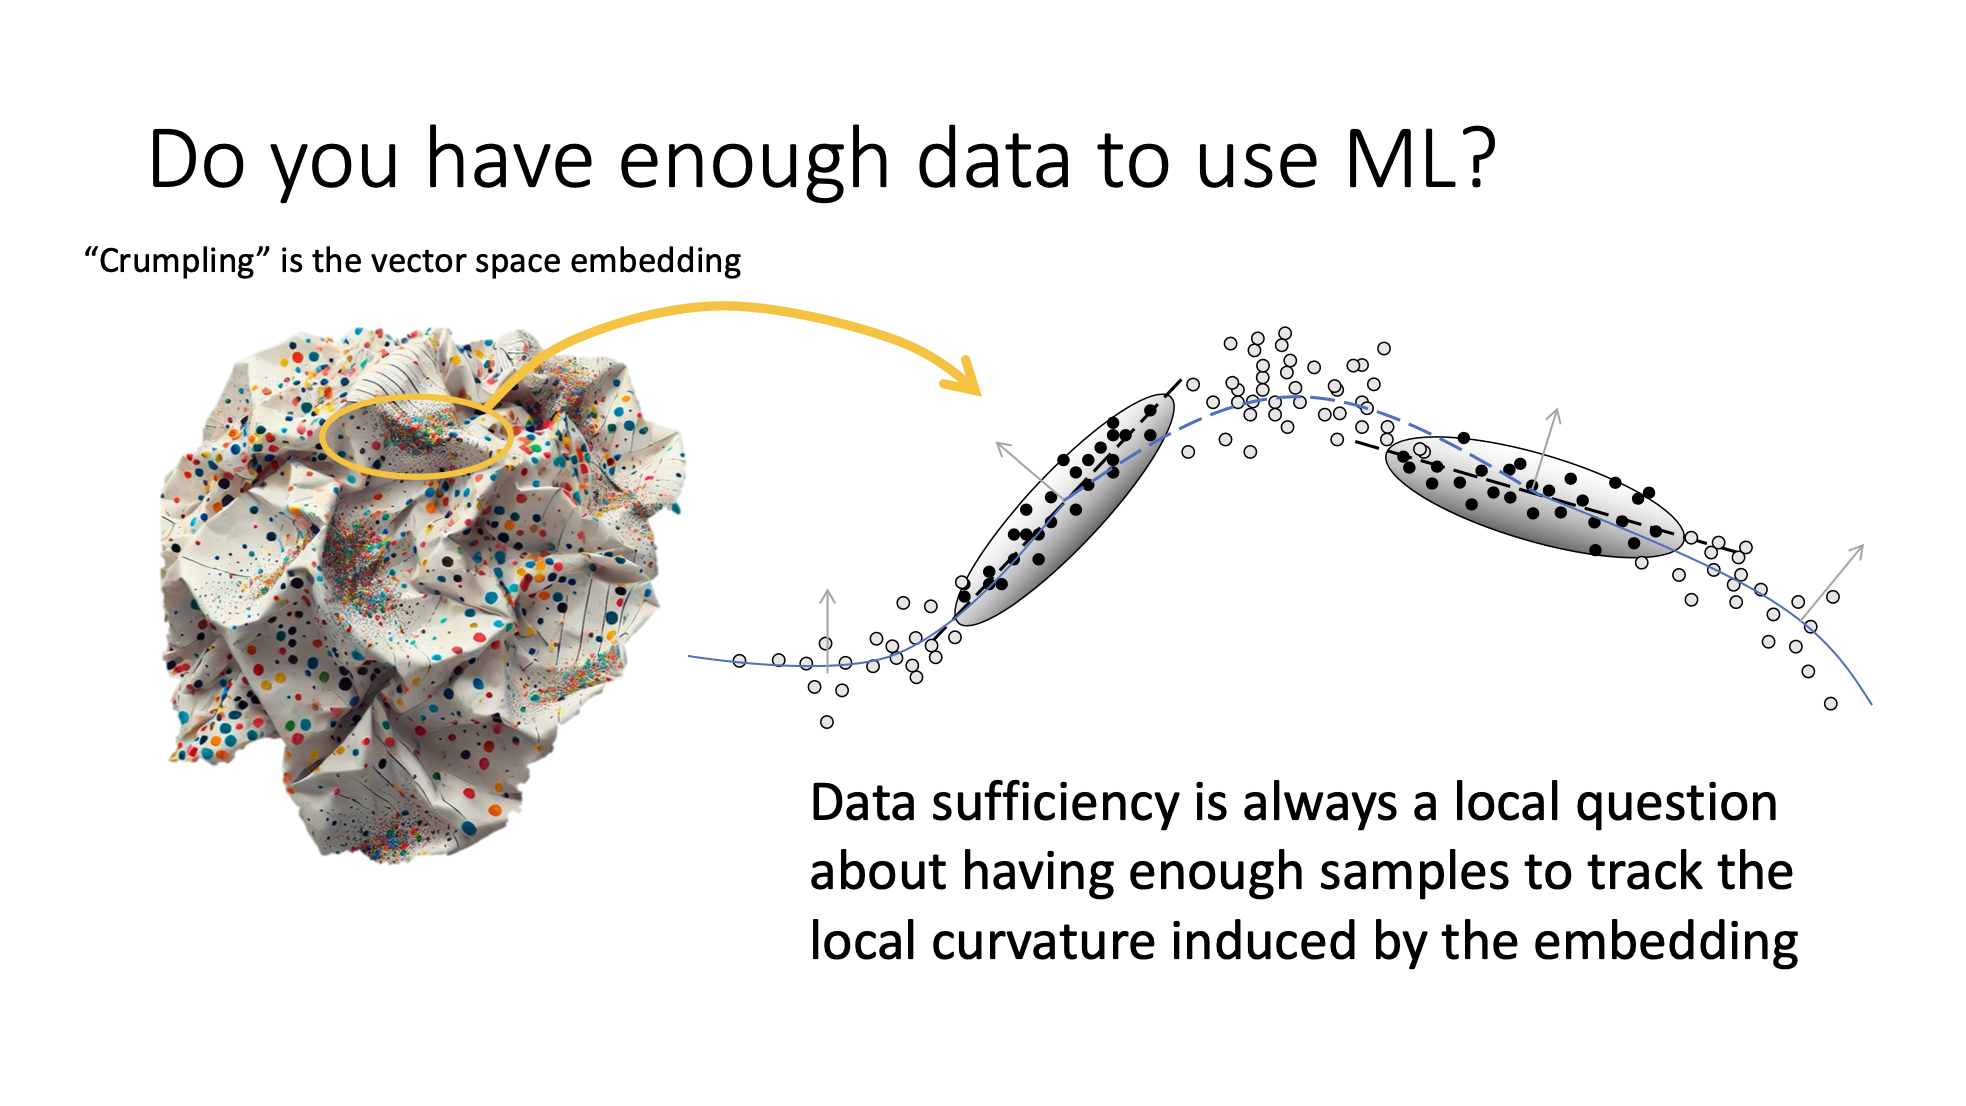
\includegraphics[width=0.8\textwidth]{figures/B1_data_sufficiency_local_question.png}
    \caption{}
\end{figure}

\begin{figure}[h!]
    \centering
        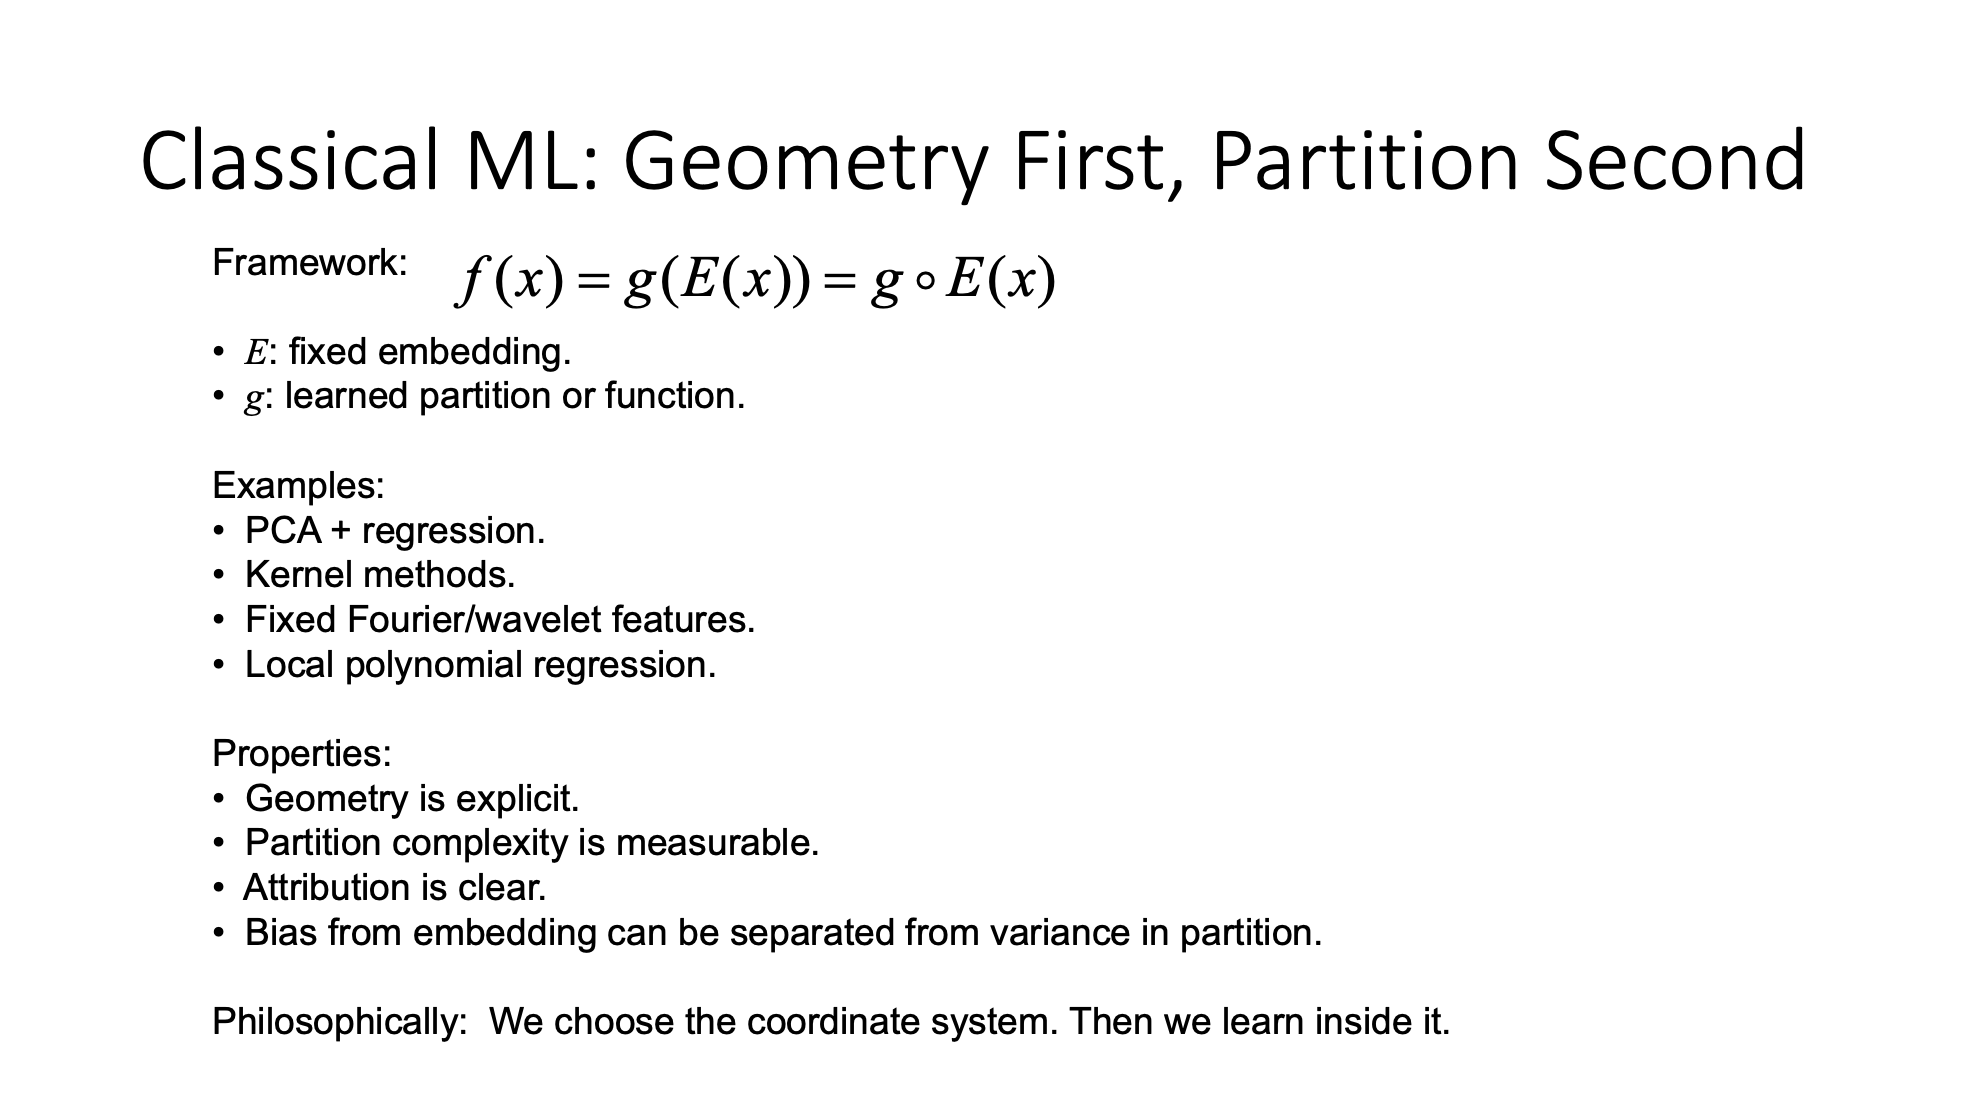
\includegraphics[width=0.8\textwidth]{figures/B1_classicalML_geometry_first.png}
        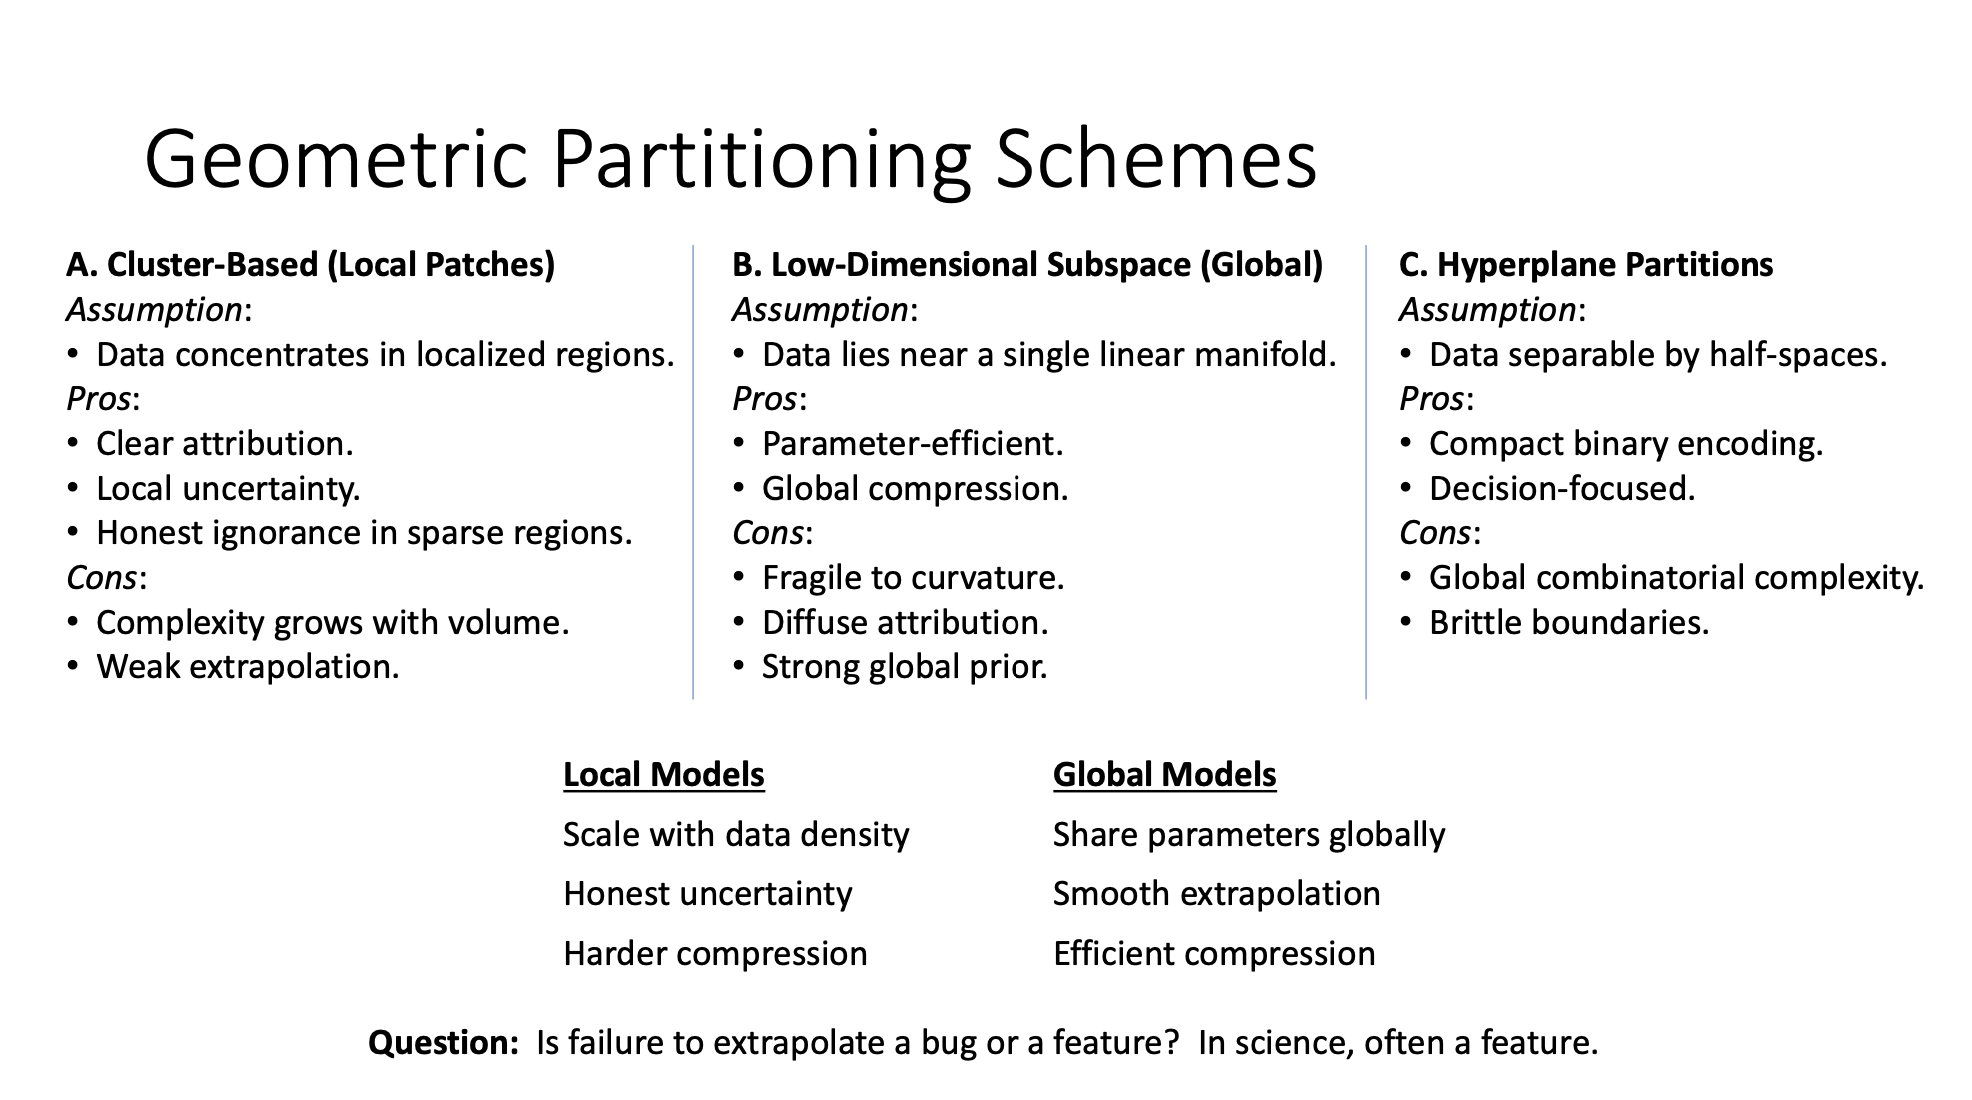
\includegraphics[width=0.8\textwidth]{figures/B1_classical_ML_geom_schemes.png}
    \caption{Classical ML: geometry first, partition second}
\end{figure}


\begin{figure}[h!]
    \centering
        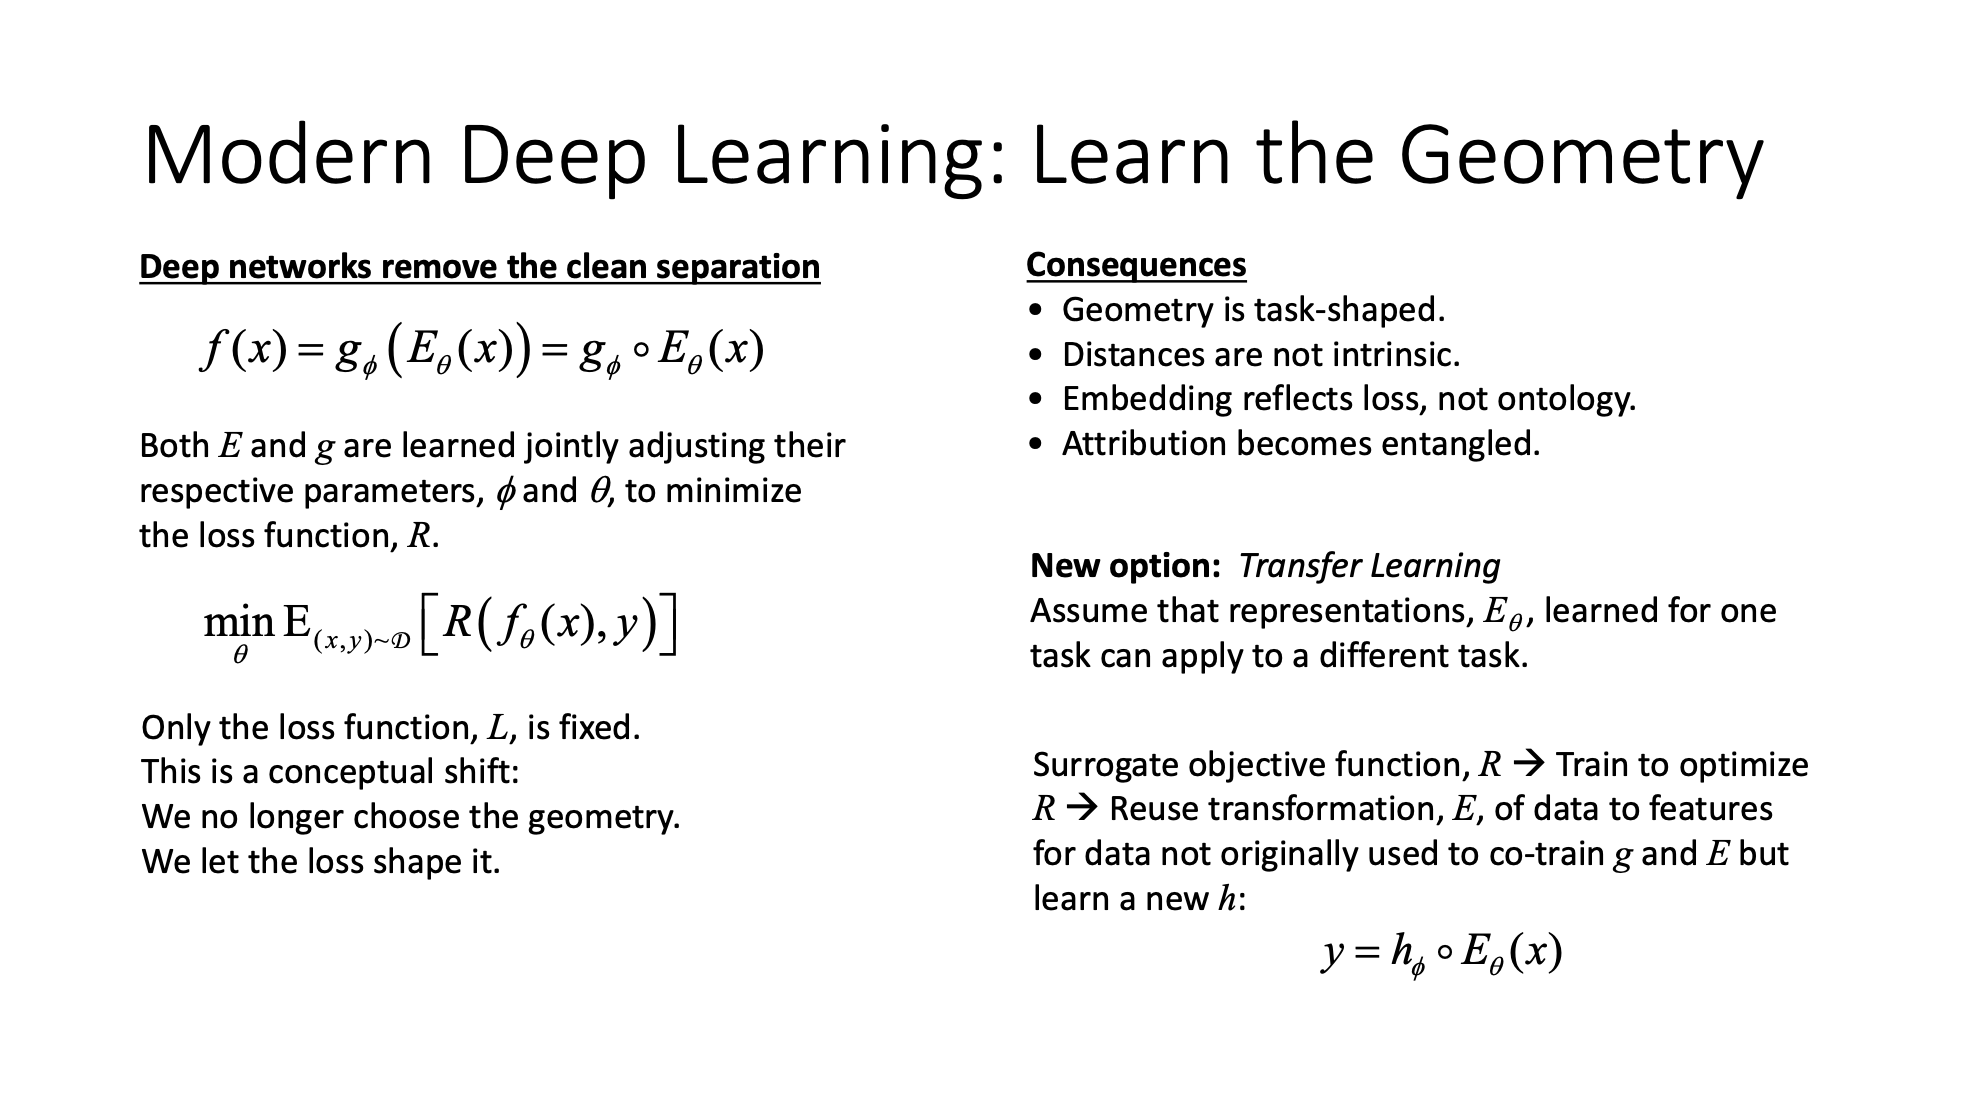
\includegraphics[width=0.8\textwidth]{figures/B1_modernML_learn_geom.png}
        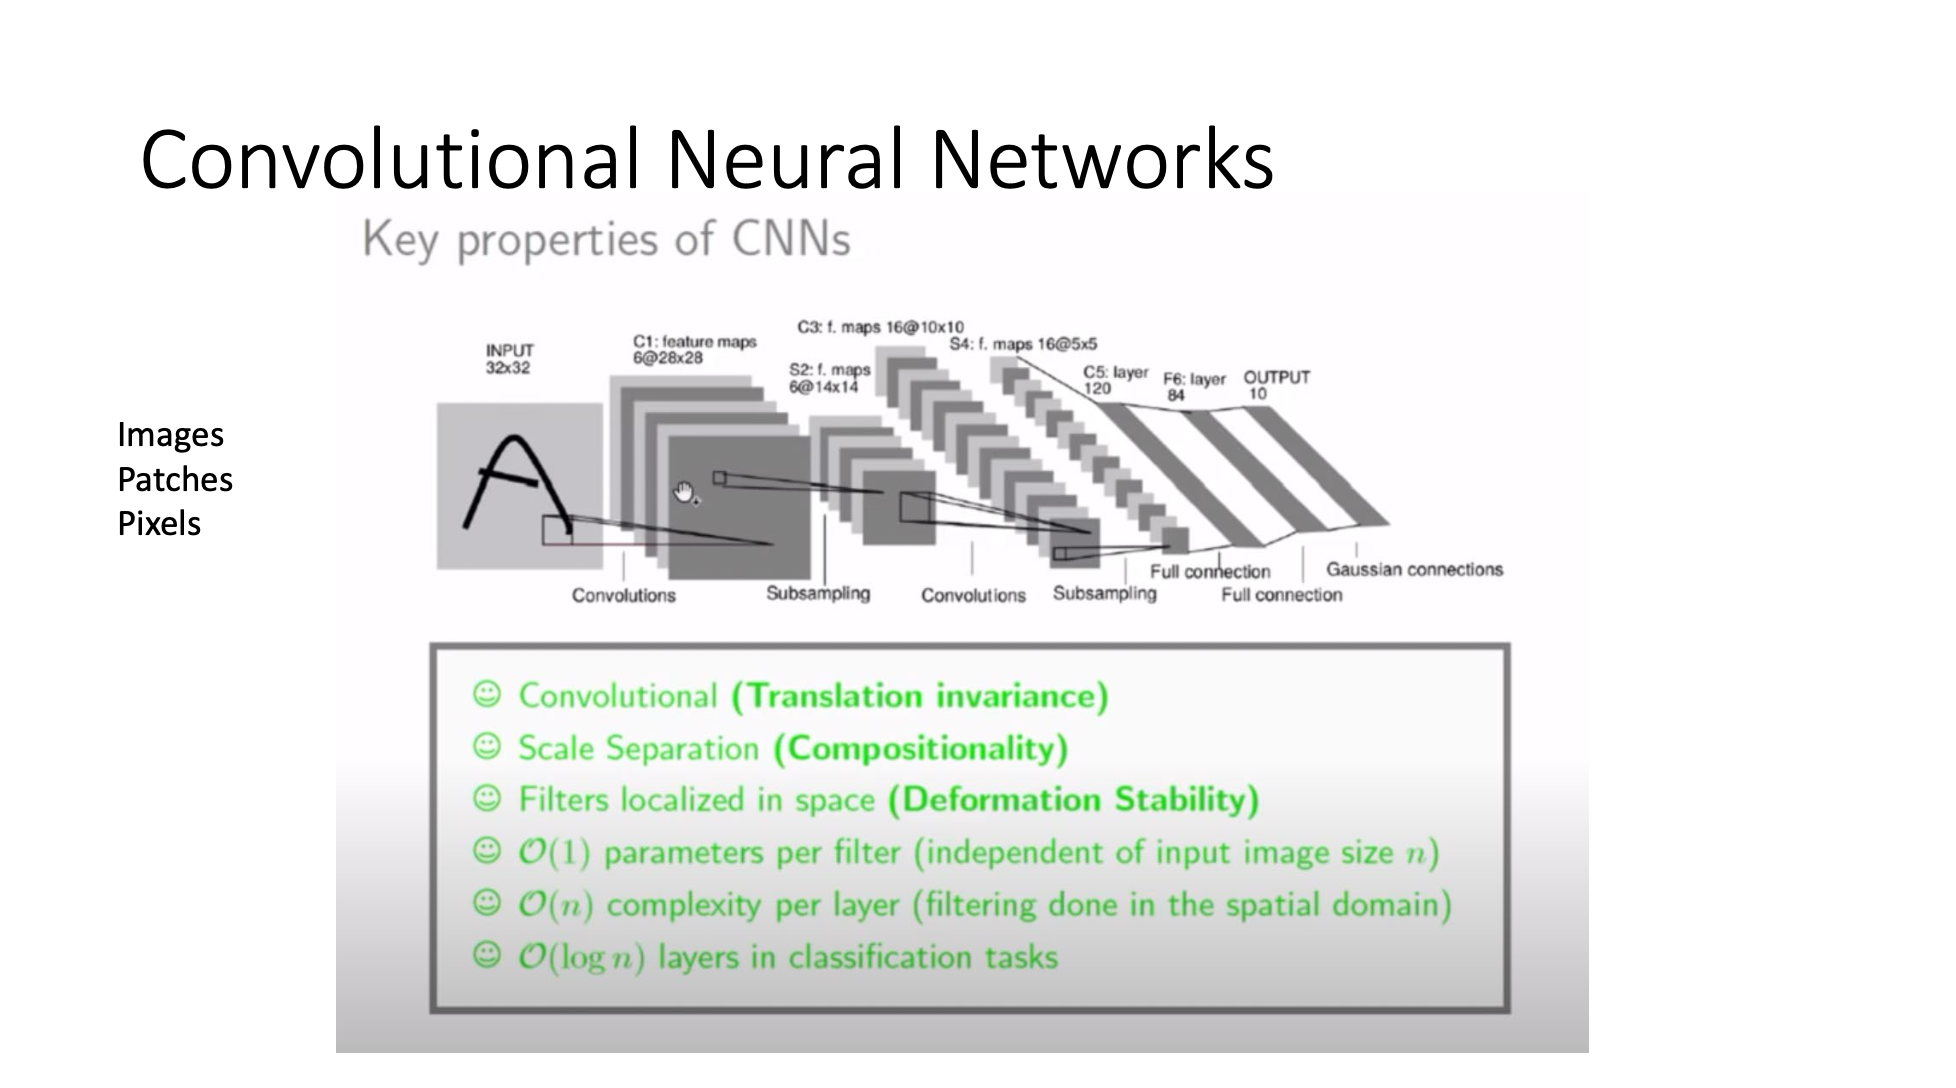
\includegraphics[width=0.8\textwidth]{figures/B1_cnns.png}
    \caption{Modern ML: learn geometry together with partition}
\end{figure}

